\chapter{Ergebnisse}

In diesem Kapitel wird die implementierte Lauferkennung ausgewertet und werden ebenfalls die Ergebnisse der Testversuchen vorgestellt und diskutiert.

Die Auswertung der Versuche beziehungsweise der Testergebnisse wird aus zeitlichen Gründen qualitativ sein und nicht quantitativ.


\section{Verifizierungsversuche}

Die bereits im \autoref{ab:Versuchsplanung} aufgelistete Versuchsszenarien wurden alle mindestens einmal getestet. Einige Testszenarien sind mit zwei Testdurchläufe durchgeführt.
Nach der Durchführung der Verifizierungsversuche werden die Ergebnisse analysiert und diskutiert. 

Die Lauferkennung ist ein großer Teil dieser Arbeit und wird demnächst mit den tatsächlichen Daten (Ground Truth) sowie die von Google integrierte Aktivitäts\-erkennung verglichen.
\section{Lauferkennung}

In der \autoref{fig:Speed_Groundtruth_MotionClass_GoogleMD_Compare} werden die verschiedenen Methoden der Aktivitätserkennung sowie die Geschwindigkeit in der obersten Grafik über die Zeit dargestellt.

Die zweite Grafik zeigt die tatsächliche Aktivitätsdaten (Ground Truth), die in vier Klassen (\autoref{fig:Lauferkennung_Klassentabelle}) unterteilt sind. Die Aktivitätsbereiche sind auch mit vertikalen roten Linien optisch unterteilt, die auch in anderer Grafiken sichtbar sind, damit diese einfach und schnell zugeordnet werden können. Bei der Sekunde \SI{460}{\second} sowie \SI{500}{\second} ist die Versuchsperson vom Motorrad ab- oder aufgestiegen, deswegen werden diese zwei Stellen mit \glqq No Motion\grqq{} klassifiziert. Ab der Sekunde \SI{556}{\second} gibt es keine Videoaufnahme mehr und wurde als \glqq Undefined\grqq{} eingetragen.

In der dritten Grafik ist die Ausgabe der im Rahmen dieser Arbeit implementierten Lauferkennung beziehungsweise Aktivitätserkennung abgebildet. 
Es ist zu bemerken, dass die Lauferkennung ein sehr große Übereinstimmung mit den Ground Truth hat. Laufen sowie Fahren werden dadurch gut erkannt. Das Auf- und Absteigen bei den Sekunden \SI{465}{\second} und \SI{508}{\second} werden die \glqq No Motion\grqq{}-Klasse vom Lauferkennung-Model vergeben.

Die letzte Grafik stellt die Ausgabe der im Smartphone integrierten Aktivitäts\-erkenn\-ung dar, die für diese Auswertung in die gleiche Klassifizierung aus der \autoref{fig:Lauferkennung_Klassentabelle} umgerechnet wird.

\begin{figure}
	\centering
	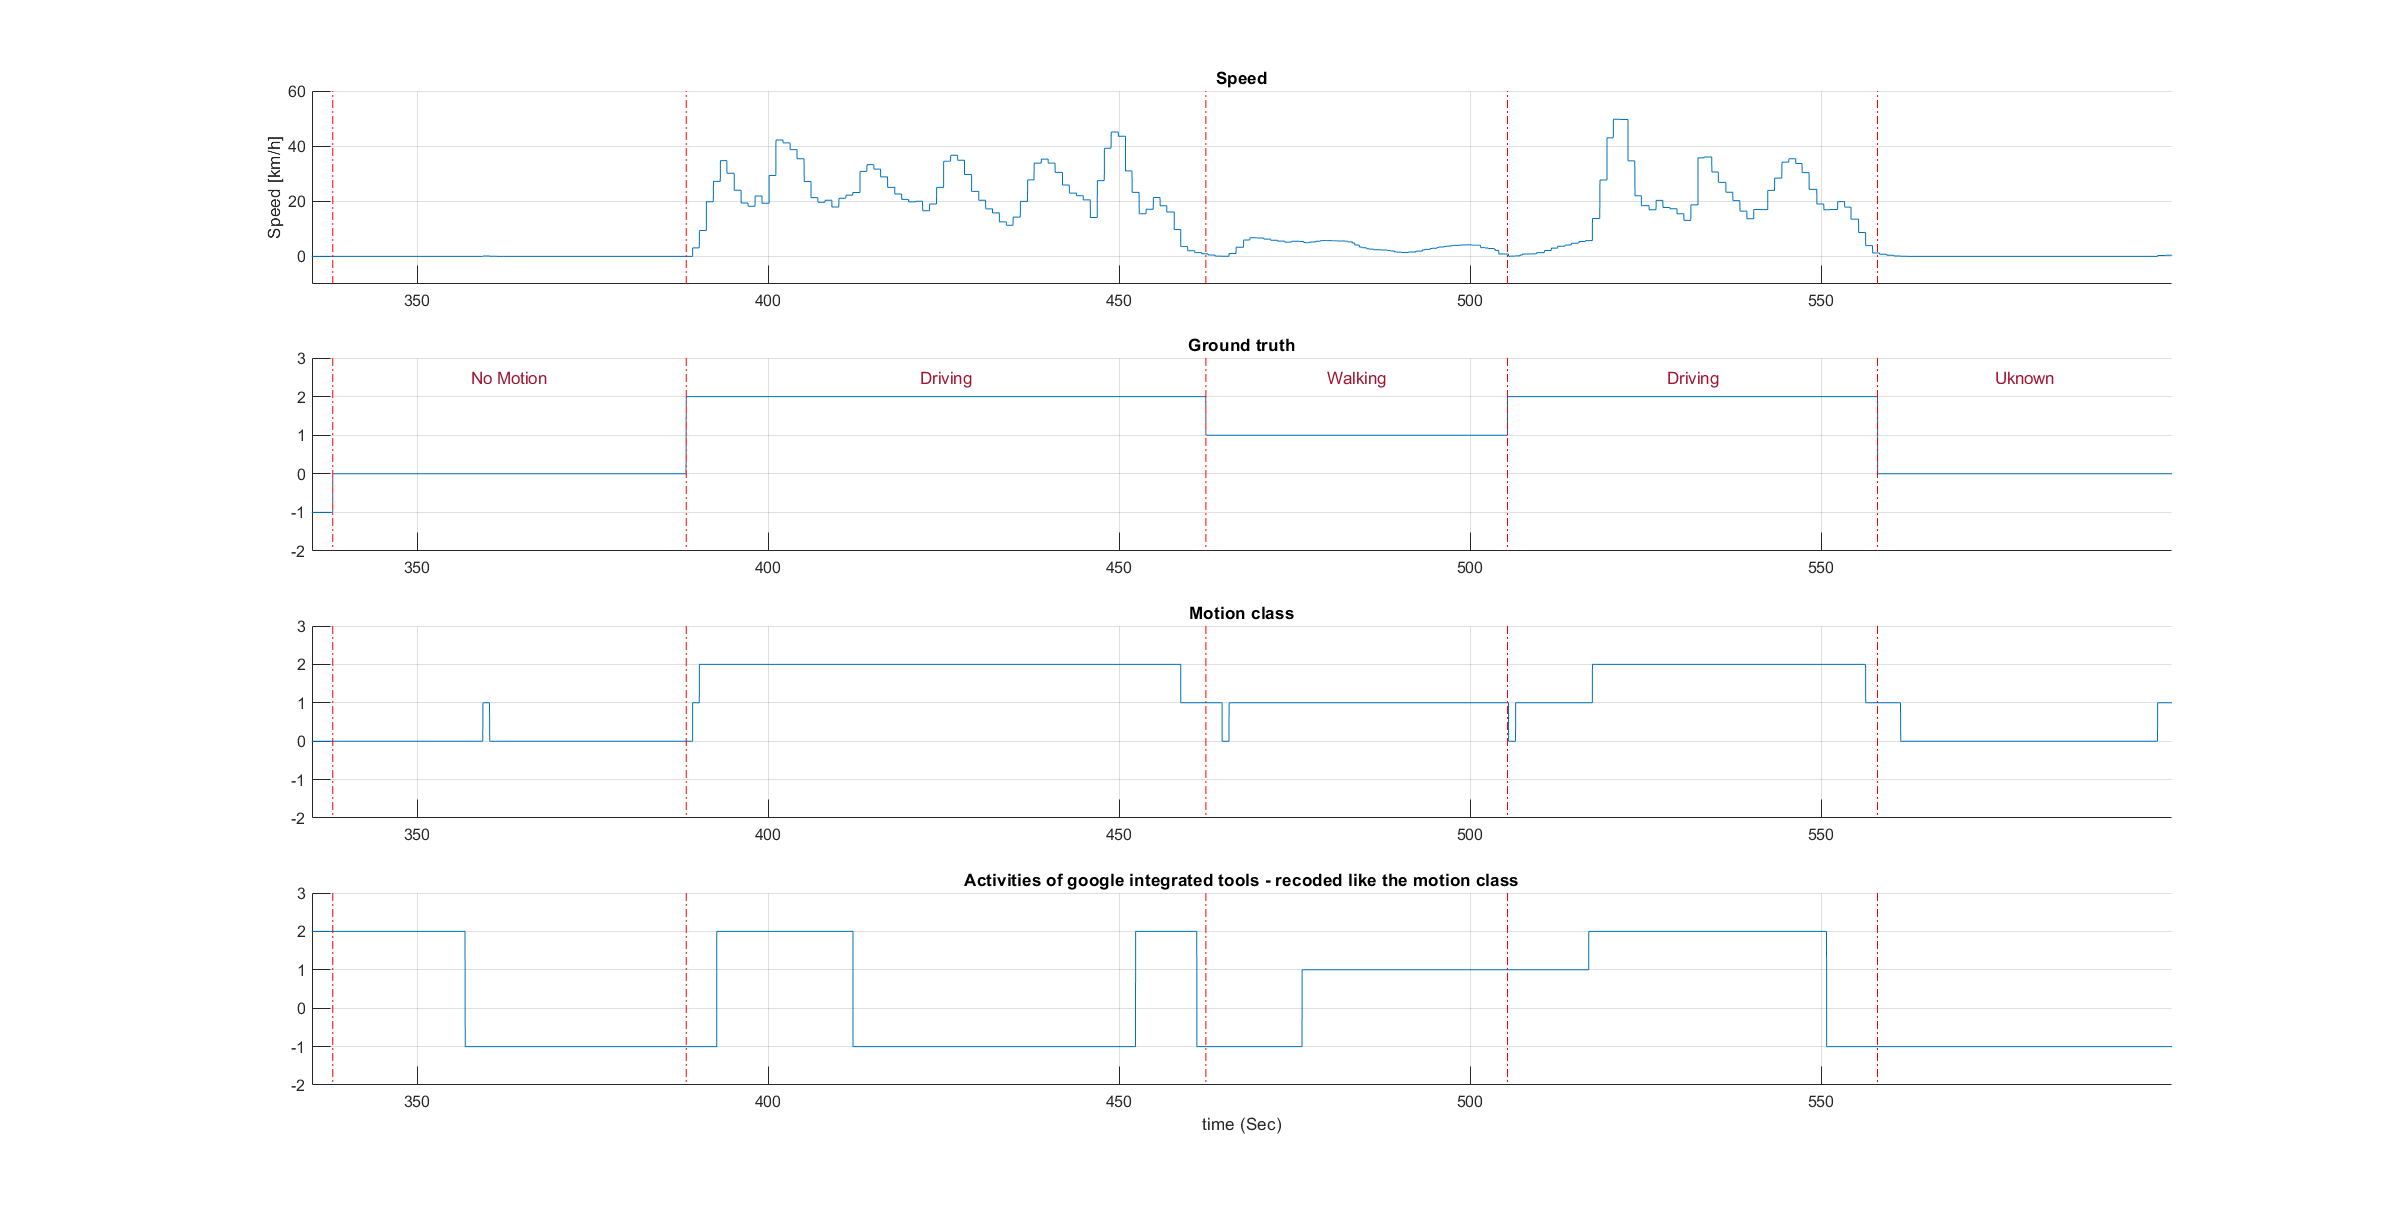
\includegraphics[width=\linewidth]{Bilder/Speed_Groundtruth_MotionClass_GoogleMD_Compare.png}
	\caption{Ergebnis des Lauferkkennungsmodells}
	\label{fig:Speed_Groundtruth_MotionClass_GoogleMD_Compare}
\end{figure}

\begin{figure}
	\centering
	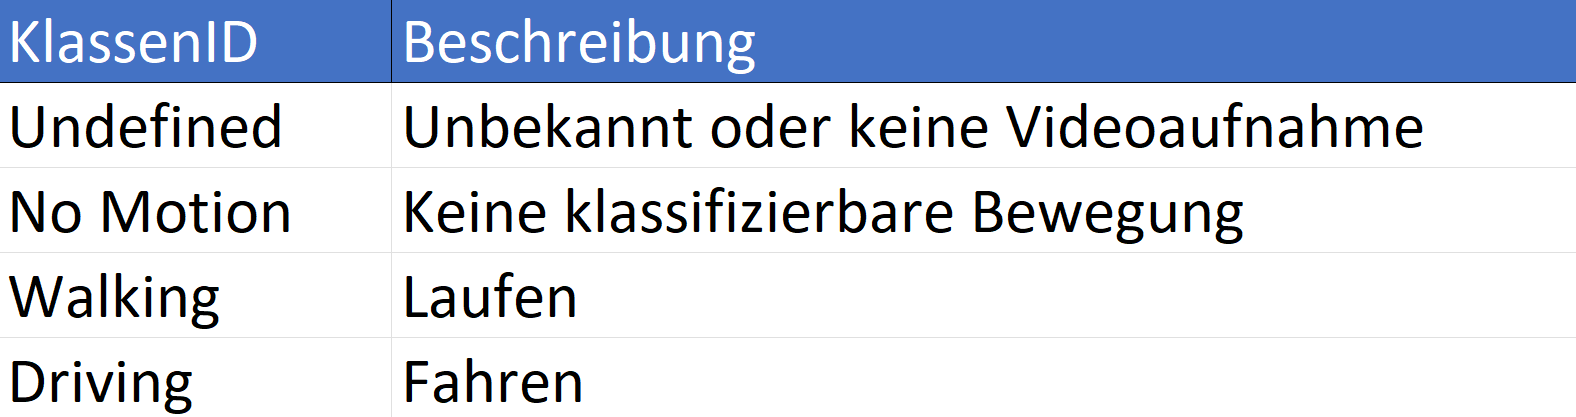
\includegraphics[width=0.6\linewidth]{Bilder/Lauferkennung_Klassentabelle.png}
	\caption{Beschreibung der Klassen in der Grafik \autoref{fig:Speed_Groundtruth_MotionClass_GoogleMD_Compare}}
	\label{fig:Lauferkennung_Klassentabelle}
\end{figure}

Aus der \autoref{fig:Speed_Groundtruth_MotionClass_GoogleMD_Compare} ist letztendlich zu bemerken, dass die Aktivitäts\-erkenn\-ung durch das implementierte Model gute Ergebnisse liefert, die mit der Wahrheit sehr gut übereinstimmt. Im Vergleich zu der Google-Aktivitäts\-erkenn\-ung (unterste Grafik) hat das Model eine wesentlich bessere Aussage getroffen. Die implementierte Aktivitätserkennung verbraucht keine große Rechenzeit (ca. $2$ bis $3$ Sekunden) und erfolgt in Echtzeit mit einer kleinen Verzögerung (ca. \SI{2,5}{\second}), da die FFT erst durchführbar, wenn \SI{256}{\second} vorhanden sind.



\section{Verschiedene Fahrerpositionierung}
Die \autoref{fig:Speed_Groundtruth_MotionClass_GoogleMD_Compare} dient zur Auswertung des ersten Testszenarios aus der \autoref{fig:TestSzenarienZusammenfassung}, in dem die Person während einer Fahrt auf der Fußraste des Motorrads für paar Sekunden steht und wieder sitzt. Das Ziel dieses Tests ist zu prüfen, ob die Änderung der Fahrerposition während einer Fahrt zur falschen Alarmauslösung führt.

Diese Darstellung zeigt die Geschwindigkeit, die Fahreraktivität (Fahren/Laufen), die Fahrerposition sowie die Winkeländerung über die Zeit.

Die Geschwindigkeit (blau) sowie die während der Fahrt Alarmauslösungen (lila) sind in der ersten Grafik abgebildet.
Die zweite Grafik stellt die tatsächliche Fahrerposition (Ground Truth) über die Zeit dar, die in drei Klassen (Sitzen, Stehen oder unbekannt) unterteilt sind.
Die Fahrerpositionsbereiche sind ebenfalls durch vertikale rote Linien optisch geteilt, die auch in anderer Grafiken sichtbar sind, damit diese einfach und schnell zugeordnet werden können.
In der Zeitbereich zwischen \SI{465}{\second} und \SI{505}{\second} ist die Versuchsperson gelaufen, deswegen lautet die Klassifizierung \glqq Unbekannt\grqq{}, da die gedachte Klassen so ein Fall nicht abdecken.

In der dritten Grafik sind die tatsächliche Aktivitätsdaten (Ground Truth), die in vier Klassen (\autoref{fig:Lauferkennung_Klassentabelle}) unterteilt sind. Die Aktivitätsbereiche sind auch mit vertikalen roten Linien optisch unterteilt. Beim Ansehen der zweiten und dritten Grafik wird einen guten Überblick über die Fahrt verschafft. Zwischen der Sekunden \SI{388}{\second} und \SI{459}{\second} fand eine Fahrt statt, während dieser ist der Fahrer zwischen der Sekunden \SI{410}{\second} und \SI{433}{\second} gestanden.

Die Kurve aus der letzten Grafik zeigt die Winkeländerung des Smartphones im Vergleich zur ursprünglichen Position nach der Kalibrierung. Aus der Darstellung ist die Winkeländerung während der ersten Fahrt, als die Fahrerposition sich verändert hat, sehr gut sichtbar. Das Laufmuster ist in diesem Signal zwischen \SI{465}{\second} und \SI{500}{\second} ebenfalls gut erkennbar.

\begin{figure}[H]
	\centering
	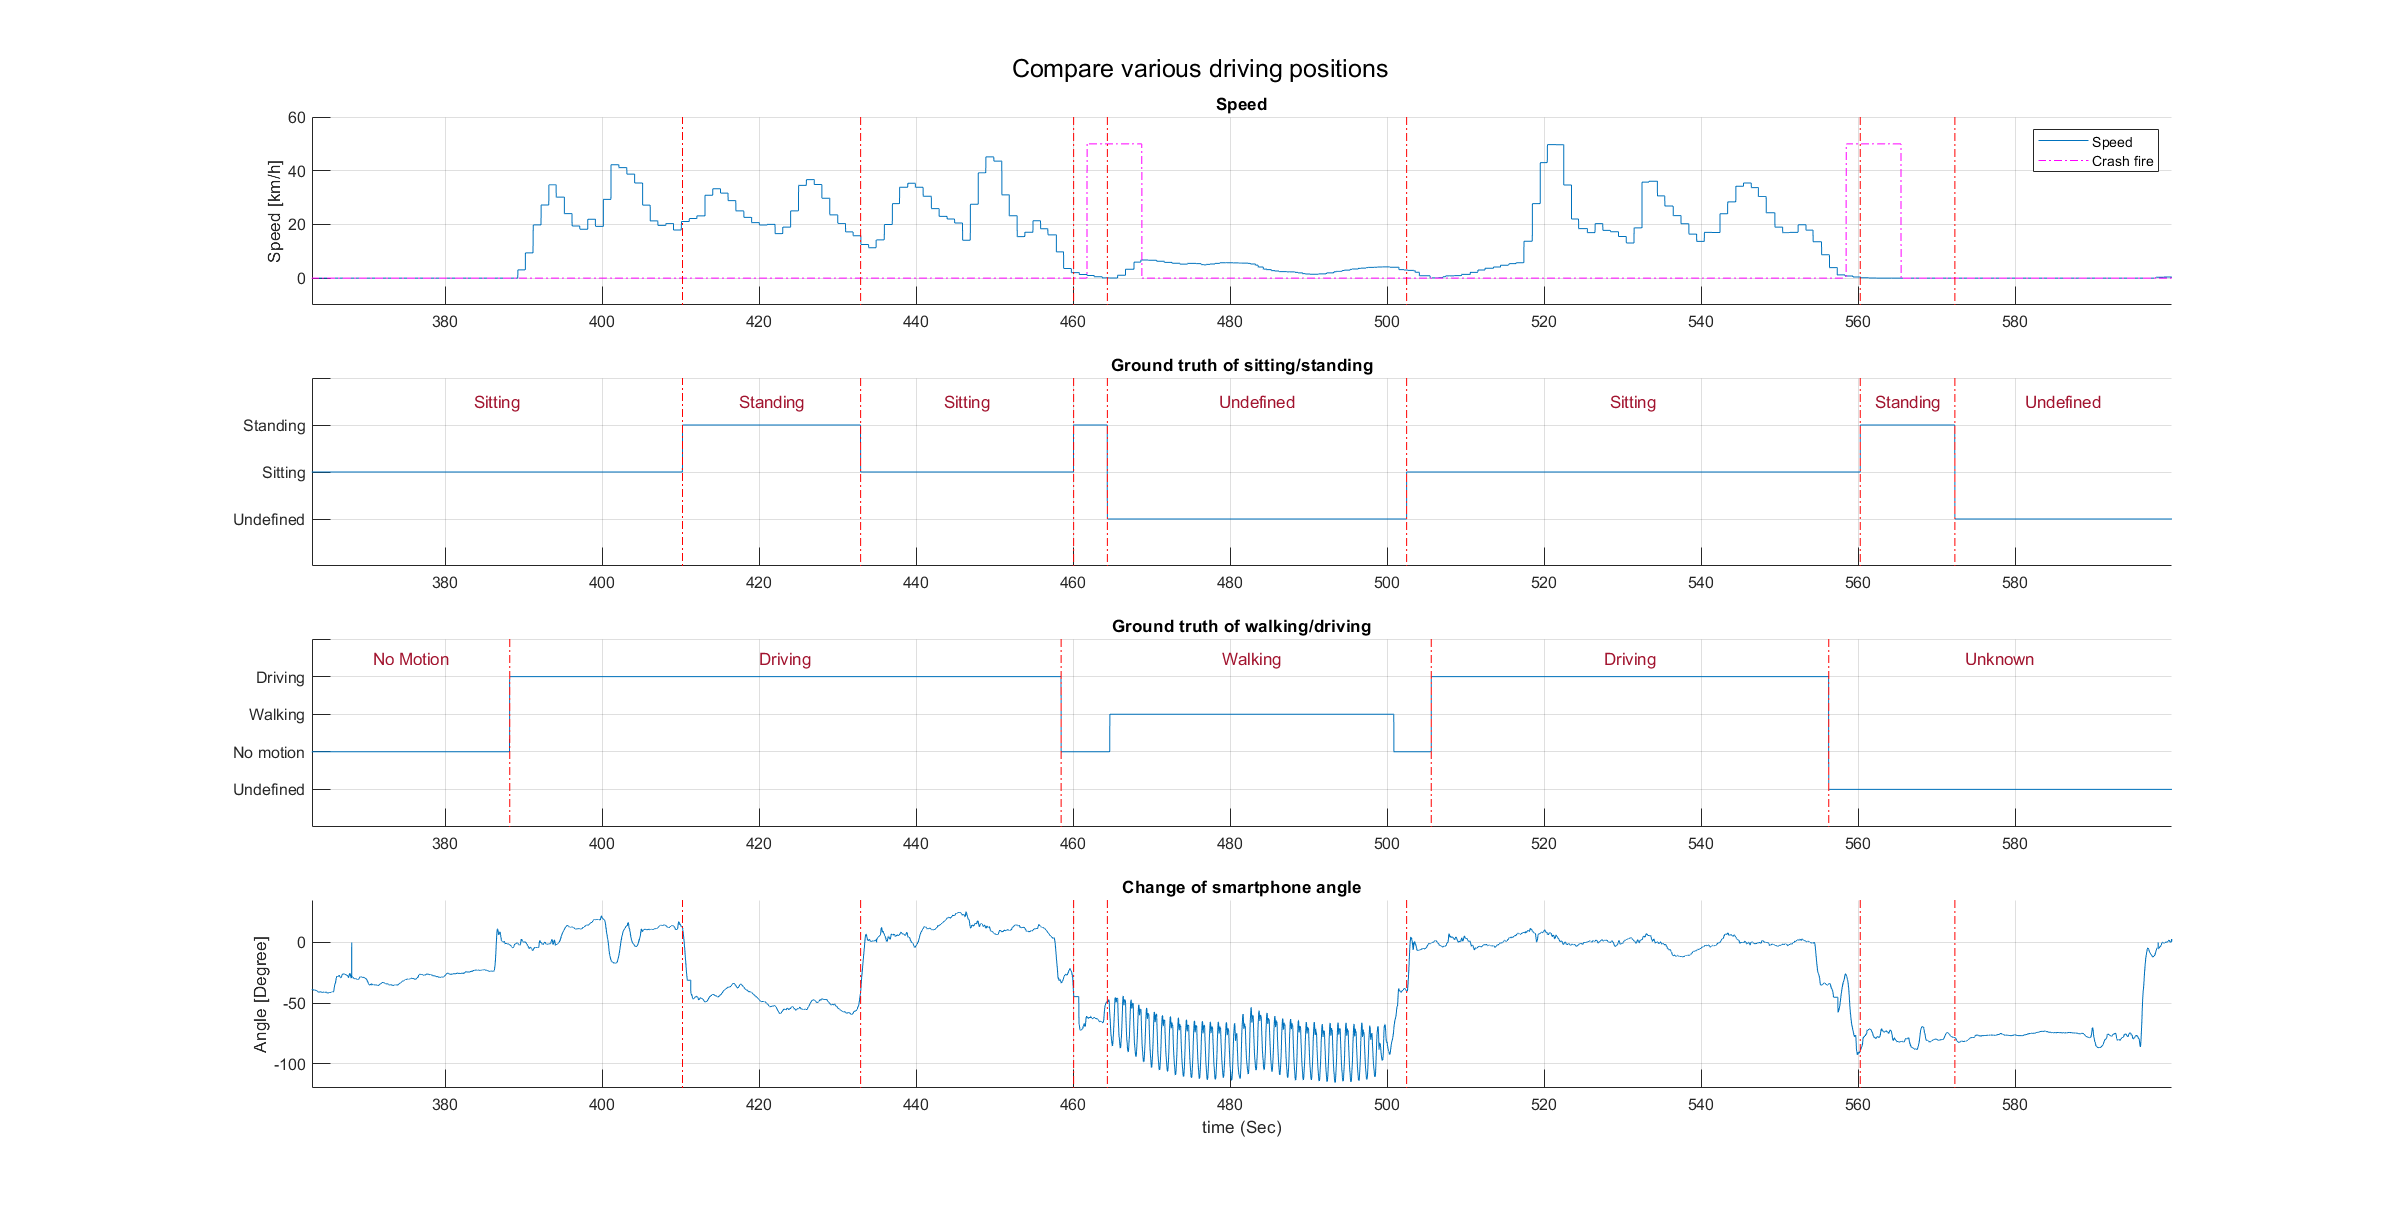
\includegraphics[width=\linewidth]{Bilder/Speed_Groundtruth_WalkStand_Compare.png}
	\caption{Zeitlicher Verlauf der Geschwindigkeit, Ground Truth der Fahreraktivität und -Position sowie der Winkeländerung}
	\label{fig:Speed_Groundtruth_WalkStand_Compare}
\end{figure}

Es ist wichtig zu bemerken, dass die Änderung der Fahrerposition während einer Fahrt keine Fehlalarme ausgelöst hat, da die Winkeländerung in so einem Fall nicht genug groß ist, um das \glqq TipOver\grqq{}-Model zu aktivieren. Beim Absteigen (ca. \SI{460}{\second} und \SI{560}{\second}) gibt es allerdings eine Alarmauslösung, da es an der Stelle sehr große Winkeländerung gibt, da der Fahrer seine Bein nach außen und hinten gestreckt hat.
\section{Anhalten}
Dieser Abschnitt diskutiert das Ergebnis des zweiten Testszenarios aus der \autoref{fig:TestSzenarienZusammenfassung}, in dem die Versuchsperson während einer Fahrt kurz anhält und sein Fuß runter setzt.

\begin{figure}
	\centering
	\psfragfig[width=\linewidth]{Bilder/0B_Anglechanging_stopping}
	\caption{Winkeländerung des Smartphones durch das Anhalten}
	\label{fig:Speed_AngleChangeCompare}
\end{figure}
Die Grafik \autoref{fig:Speed_AngleChangeCompare} zeigt die Geschwindigkeit sowie die Winkeländerung zum ursprünglichen Position nach der Kalibrierung über die Zeit.
Während des Tests war gesehen, dass der Fahrer dreimal anhält und sein Fuß runter setzt, was in der Geschwindigkeitskurve sichtbar ist (\SI{262}{\second}, \SI{315}{\second} und \SI{350}{\second}). Es wurde während des Tests keine Fehlalarmauslösung entgegen den Erwartungen gegeben. Nach tieferen Analyse ist der Grund bekannt worden.

Die Winkeländerung beträgt nicht \ang{90} sondern nur ca. \ang{20}-\ang{30} (\autoref{fig:MotorbikeDrivingStanding}). Die Person hat sein Bein beim Sitzen nicht genau horizontal sondern leicht nach Unten gebogen. Wenn der Fahrer sein Fuß runter setzt, ist diese ebenfalls nicht genau vertikal sondern leicht gebogen mit einem Winkel von ca. \ang{10}-\ang{20} zur vertikalen Strich. D.h. die Winkeländerung ist nicht über \ang{45} und sollte auch zu keinen Alarmauslösungen führen.

\begin{figure}
	\centering
	\begin{subfigure}{0.48\textwidth}
		\centering
		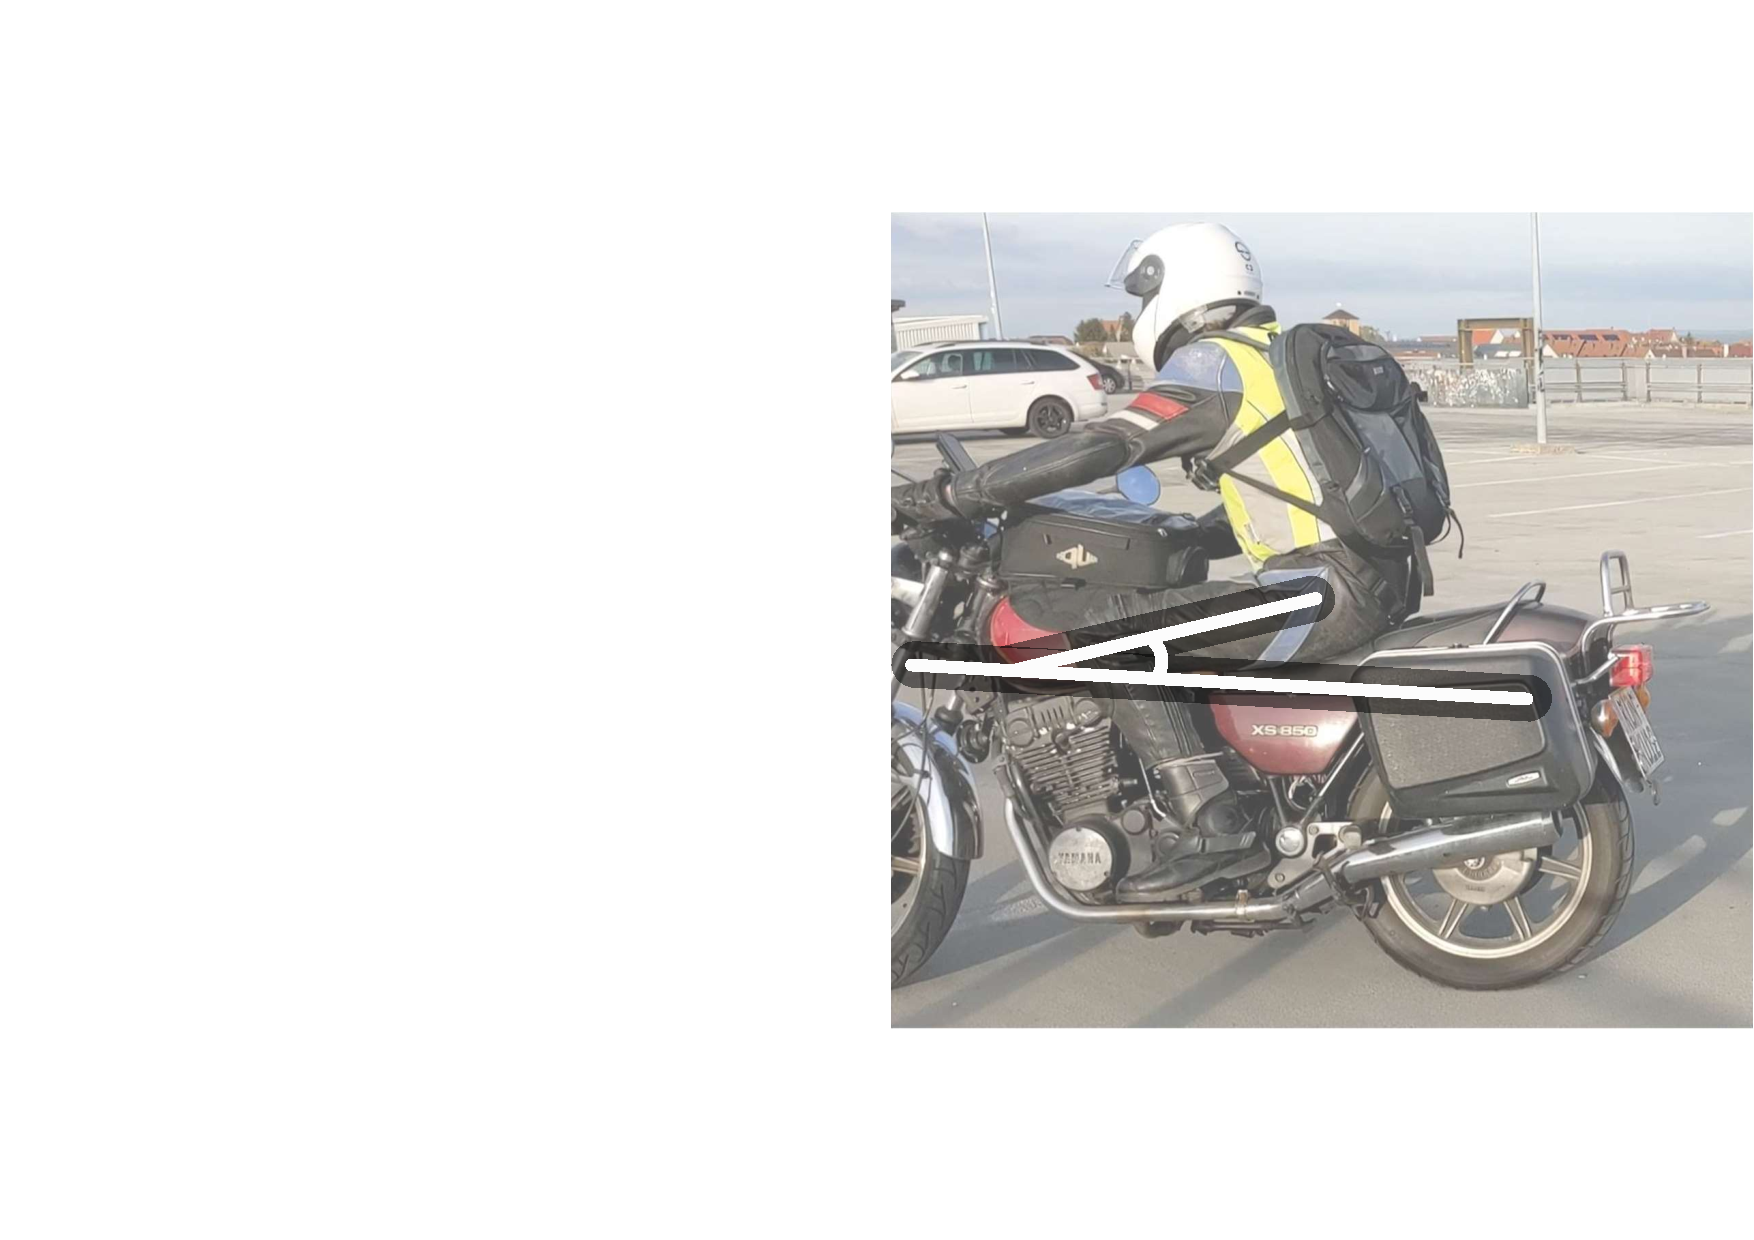
\includegraphics[width=\textwidth]{Bilder/0_Beinposition_Anhalten_Fahren.pdf}
		\caption{Beinposition während einer Fahrt}
		\label{fig:MotorbikeDriving}
	\end{subfigure}
	\hfill
	\begin{subfigure}{0.48\textwidth}
		\centering
		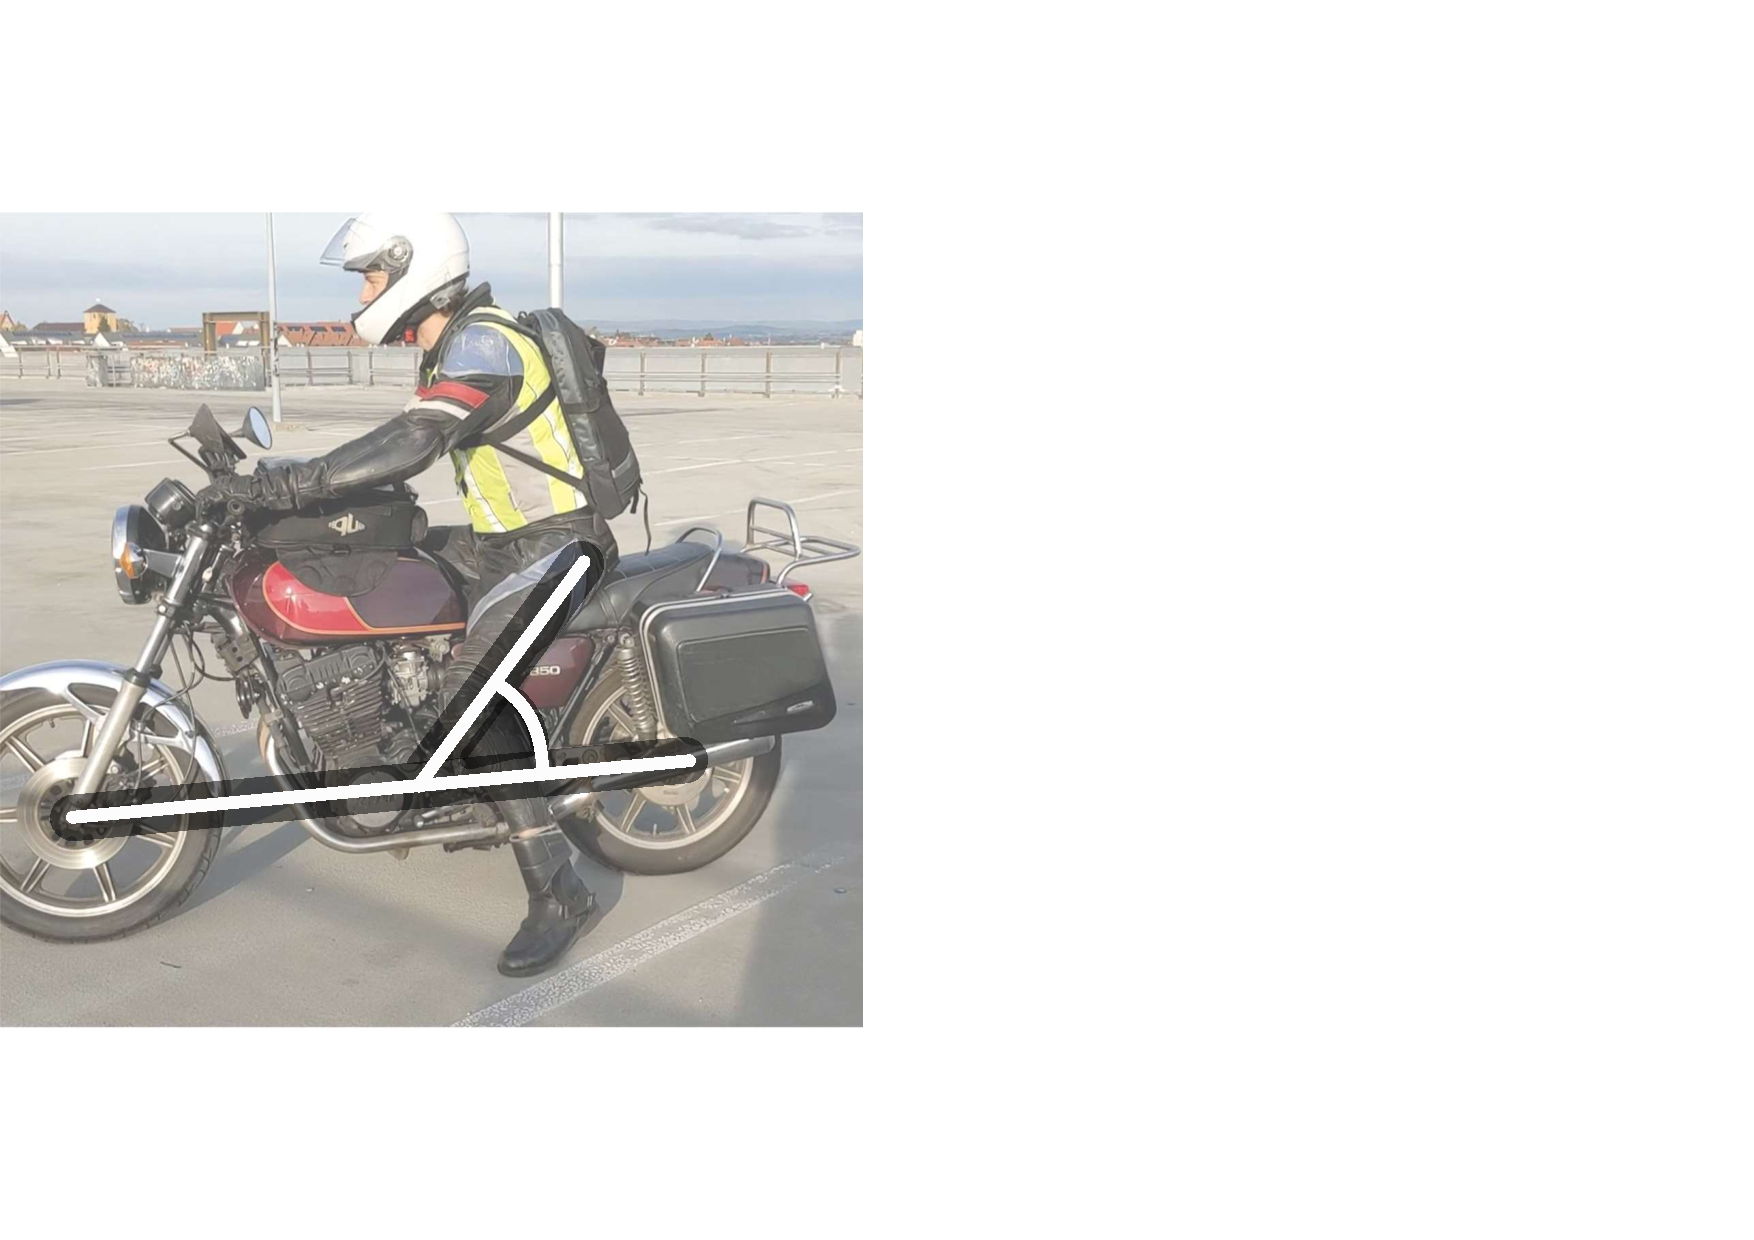
\includegraphics[width=\textwidth]{Bilder/0_Beinposition_Anhalten_Stehen.pdf}
		\caption{Beinposition Beim Stehen}
		\label{fig:MotorbikeStanding2}
	\end{subfigure}
	\caption{Beinpositionen während einer Fahrt und beim Anhalten}
	\label{fig:MotorbikeDrivingStanding}
\end{figure}


 